%!TEX root = ../Thesis.tex
\chapter{Results}

\section{Software and implementation}
This section will not discuss the details of the model implementations, but will just citrate the work required for creating the results.

Overall the results was generated with the programing language Python \cite{python}. The skip-gram (word2vec) and paragraph2vec (doc2vec) implementation is from the Python module Gensim \cite{gensim}. The Sutskever model \cite{sutskever} have not been made available as an open source module and nobody else have implemented and open sourced it. It was thus necessary to implement a framework for creating the network. For generating fast code, utilizing the GPU and deriving the backward pass, the Theano framework \cite{theano-a, theano-b} was used. From a more thorough discussion on the this implementation please see \autoref{appendix:implementation}.

As the intellectual properties for news articles are typically not addressed to the public domain, no big free corpus of news articles exists. The news articles was thus collected by crawling RSS feeds and using a previously developed heuristic\footnote{\url{https://github.com/AndreasMadsen/article}} for getting the article text and title from the HTML page.

The code for the Sutskever model implementation and generating the results is available under an MIT open source license at \url{https://github.com/AndreasMadsen/bachelor-code}.

\clearpage
%!TEX root = ../Thesis.tex
\section{Skip-gram}

The skip-gram model doesn't need to be trained as there exists a pre trained version at \url{https://code.google.com/p/word2vec/}. This pre trained version has a latent size of 300 dimensions. The weights are trained using the Google News dataset, which is about 100 billion words and unfortunately not publicly available.

The document vectors are then constructed by taking the average sum over all the word vectors. Using the full text of each article is unlikely to provide any good results, as there would be a lot of irrelevant words which would create a lot of noise. 

Instead just the title of the article is used and as an experiment the title and the subhead is also considered.

\paragraph{Document vectors} Using principal component analysis the vector representations of all the documents can be visualized in both cases.
\begin{figure}[H]
	\centering
	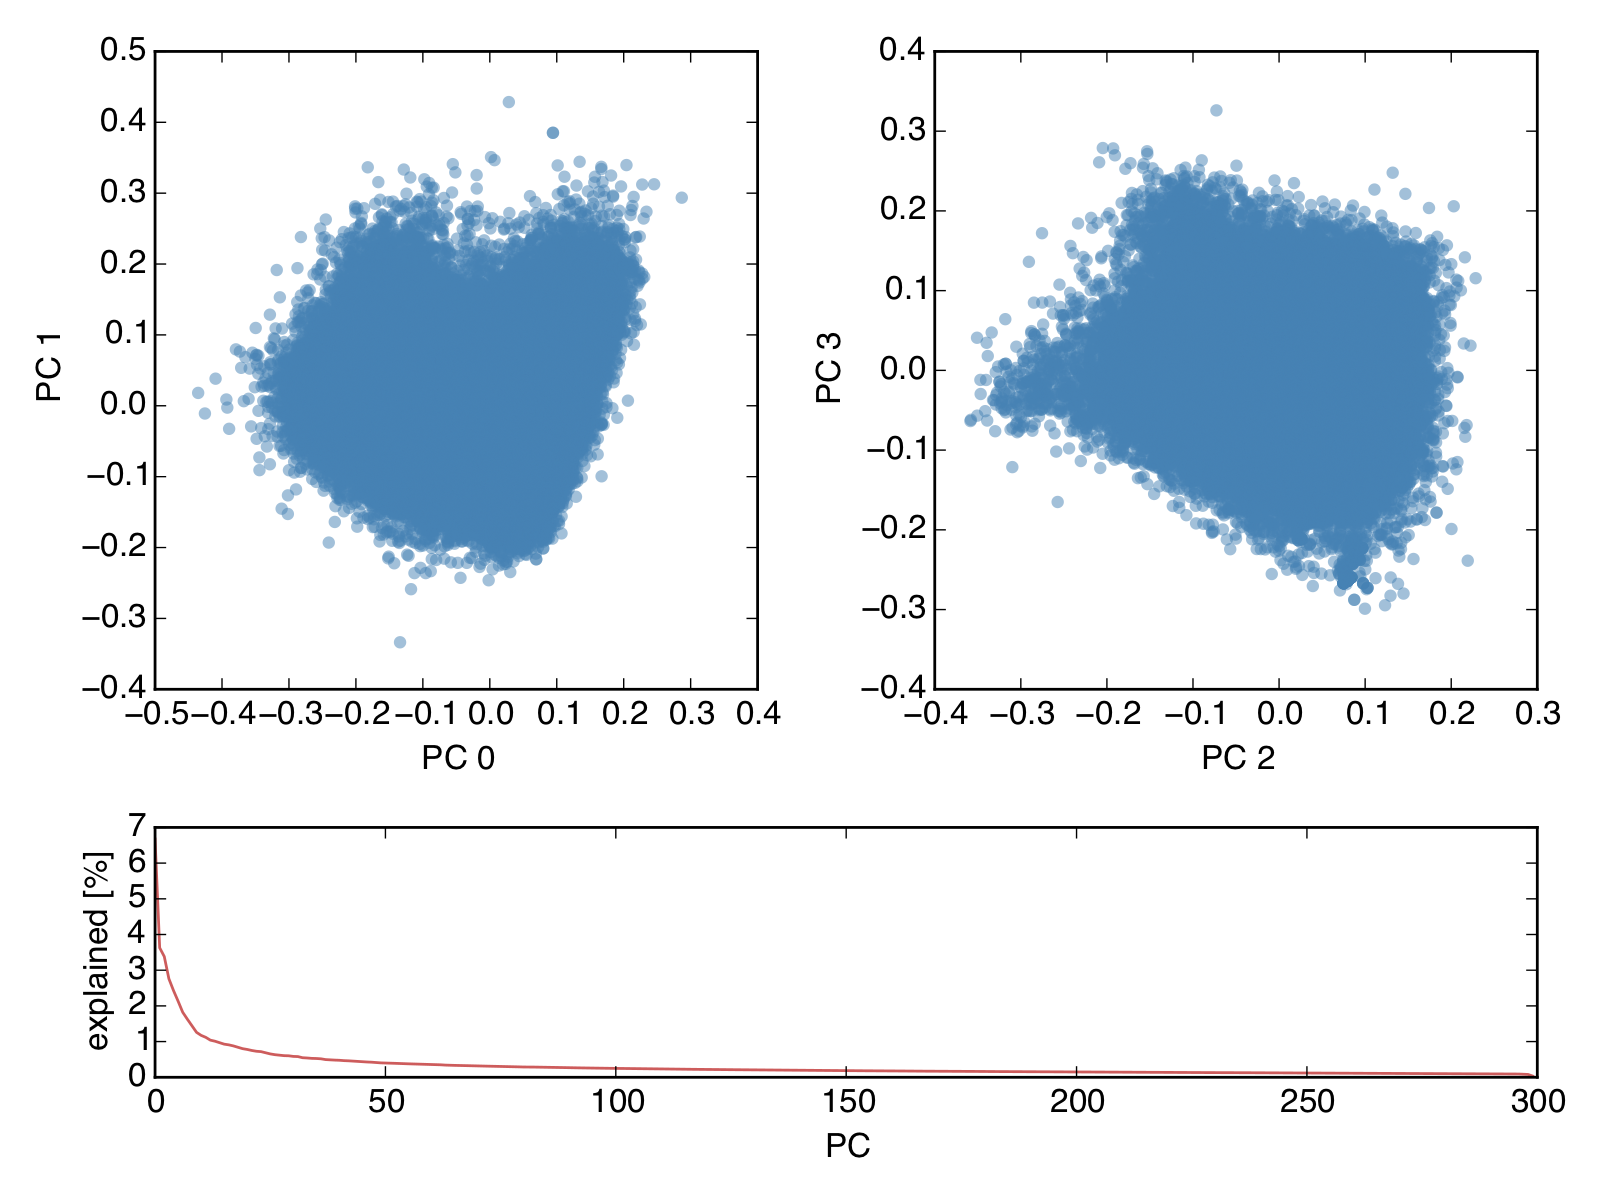
\includegraphics[width=0.9\textwidth]{results/word2vec-title-pca}
	\caption{Document vectors calculated from just the title. Explaned variance on the first 4 principal components is 16.4\%.}
\end{figure}

\begin{figure}[H]
	\centering
	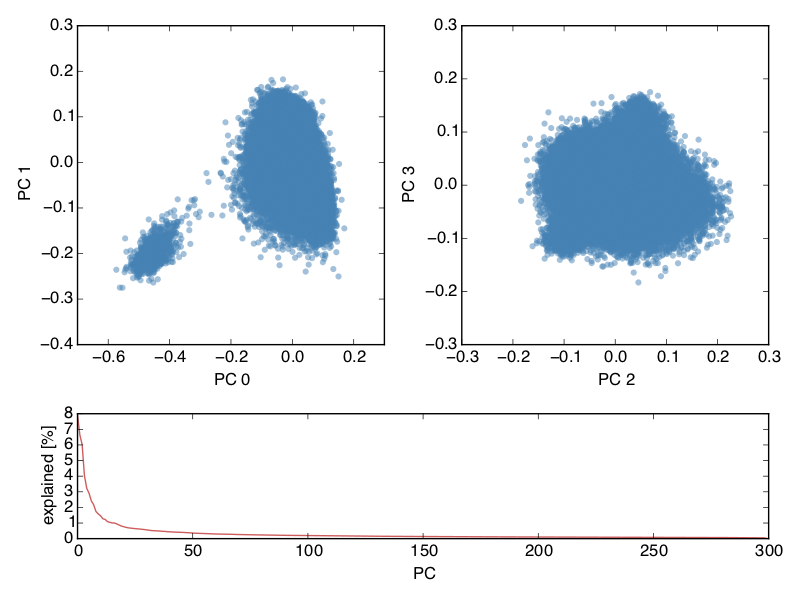
\includegraphics[width=0.9\textwidth]{results/word2vec-both-pca}
	\caption{Document vectors calculated from both title and subhead. Explaned variance on the first 4 principal components is 24.6\%.}
\end{figure}

Without any labeling of the documents the scatter plots are not very informative. The explained variance score is not very high compared to what one usually observes on raw data. This indicated the skip-gram model is somewhat effective in generating descriptive document vectors there aren't too correlated.

An interesting result is that the first principal component seams to contain two big clusters of documents. However by inspecting some of the nodes there do not appear to be any reason for this seperation.

\paragraph{Distance histogram} Since a distance measure will be used to perform the clustering, it makes sense to inspect the histogram of the distance measures. Note that only distances between nodes there are connected by the chronological connectivity matrix have been calculated.

The density estimation required for showing the histogram, also serves the purpose of providing the basis for calculating a somewhat consistent threshold across the diffrent experiments. The threshold $t$ is chosen a the $0.1 \%$ percentile, that is $P(distance < t) = 0.001$. This percentile was chosen qualitatively by running a few experiments, but it turns out it doesn't matter much, as the threshold is not the bottleneck of the performance.

\begin{figure}[H]
        \centering
        \begin{subfigure}[b]{0.49\textwidth}
                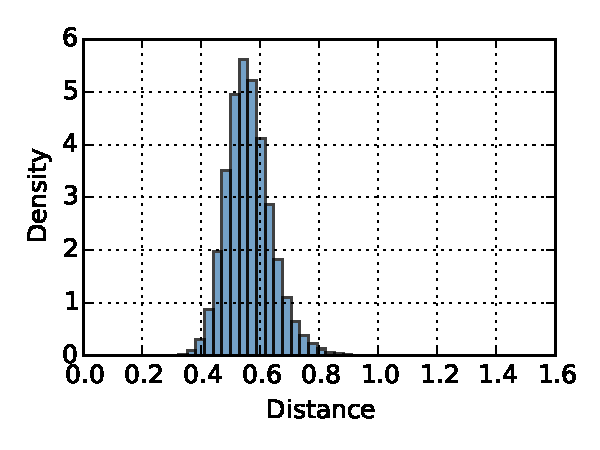
\includegraphics[width=\textwidth]{results/word2vec-title-l2-histogram}
                \caption{Euclidian distance ($t \approx 0.35$)}
        \end{subfigure}
        \begin{subfigure}[b]{0.49\textwidth}
                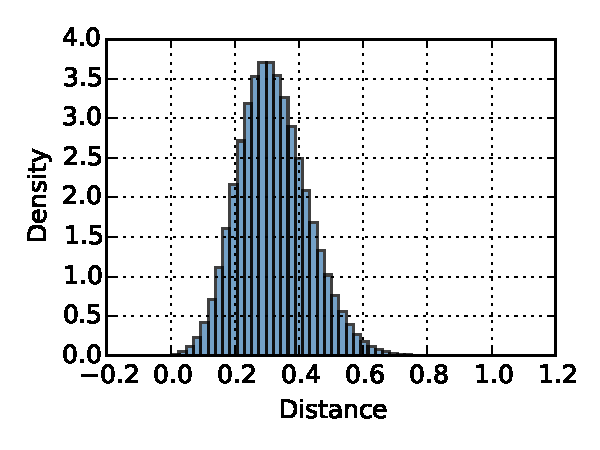
\includegraphics[width=\textwidth]{results/word2vec-title-cos-histogram}
                \caption{Cosine similarity ($t \approx 0.14$)}
        \end{subfigure}
        \caption{Histograms of the distance values using just the title for generating document vectors.}
\end{figure}
\begin{figure}[H]
        \centering
        \begin{subfigure}[b]{0.49\textwidth}
                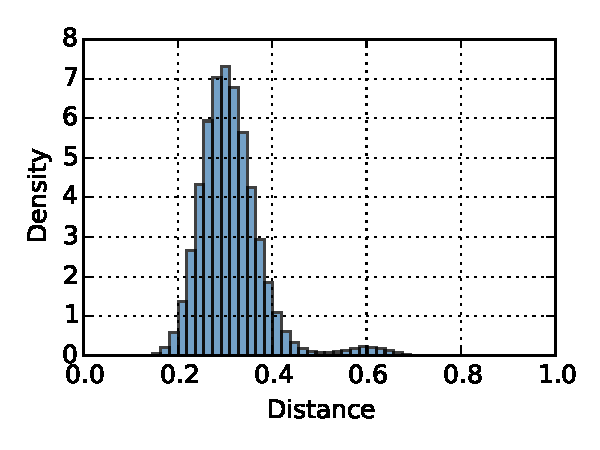
\includegraphics[width=\textwidth]{results/word2vec-both-l2-histogram}
                \caption{Euclidian distance ($t \approx 0.14$)}
        \end{subfigure}
        \begin{subfigure}[b]{0.49\textwidth}
                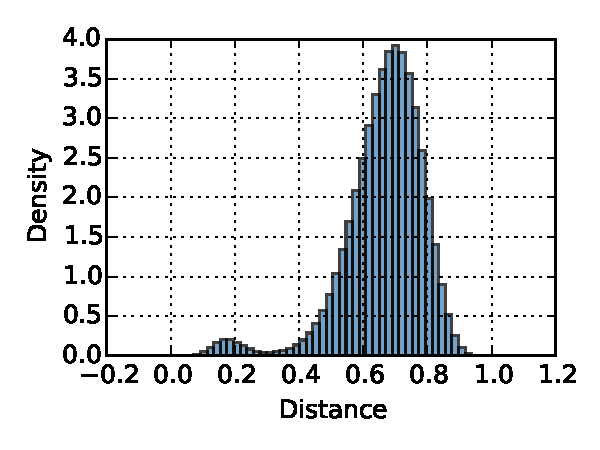
\includegraphics[width=\textwidth]{results/word2vec-both-cos-histogram}
                \caption{Cosine similarity ($t \approx 0.092$)}
        \end{subfigure}
        \caption{Histograms of the distance values using both title and subhead for generating document vectors.}
\end{figure}

The histograms shows the distances are approximately normally distributed. This is not very surprising as the both the euclidian distance and cosine similarly involves a large sum and thus have relations to the central limit theorem.

\paragraph{Inspecting clusters}  None of the 4 variations gives particularly good results. They all cluster the documents such that there is a ridiculously huge amount of unique articles. This alone could indicate the threshold is too small. However simultaneously they all have cluster really big clusters, with up to $31478$ documents in one case. Because there exists clusters that either way to big or way to small, the threshold is not the problem. It is the skip-gram model or perhaps the clustering method there causes the bad results.

\begin{table}[H]
\centering
\begin{tabular}{r|l l l l l l }
size & 1 & 2 & 81 & 318 & 715 & 17023 \\ \hline
amount & 81857 & 3 & 1 & 1 & 1 & 1
\end{tabular}
\caption{Example of the cluster size distribution. In this case both title and subhead was used for generating document vectors and cosine similarity was used for clustering. Note that using euclidian distance yields way more reasonably sized clusters.}
\end{table}

It should be noted that some clusters do provide good results:

\begin{table}[H]
\centering
\begin{tabular}{r|p{10cm}}
id & title \\ \hline
 25167 & Teenage stowaway survives five-hour flight hiding in wheel of plane \\
 25354 & Survival of teenage stowaway on five-hour flight to Hawaii is medical 'miracle', say experts \\
 25140 & Teenager stowaway 'survives five-hour flight in wheel of plane' \\
 26276 & How teenage boy stowed away on plane wheel well \\
 25567 & Teenage stowaway survives five-hour flight in jet's wheel
\end{tabular}
\caption{A cluster containing articles about the same storry. Produced using euclidian distance on document vectors produced from both title and subhead.}
\end{table}
 
Similar results can be found when just looking at the title and using euclidian distance for clustering. However using cosine similarity did not yield any meaningful results, independent of whether or not the subhead was included. This is wired as the skip-gram papers \cite{word2vec-comparing, word2vec-details} uses the cosine similarity for finding similar words. It could be because cosine similarity is usually used in a context where the length of the vector isn't important. But in this case having a big length could indicate how extreme the article is in its language, which could be created to the story. 

\clearpage
%!TEX root = ../Thesis.tex
\section{Paragraph2vec}

The pre trained skip-gram model can't be used as basis for training the paragraph2vec model, as it don't contain the weights used in the hierarchical softmax, nor does it contain the structure of the Hoffman tree. Because of this both word and document vectors was trained using the gensim implementation.

The model was trained using the full text of all 273813 articles. The dimensionality of the word and document vectors was set to 500. Furthermore the model was trained over 10 epochs, with an initial learning rate of 0.025, which then decreased with 0.002 for each epoch. The vector representations of the chronologically first 100000 articles was then extracted from the final model.

Note that gensim doesn't provide any way of inspecting the loss function directly which is why no such curve is shown here.

\paragraph{Document vectors} Using principal component analysis the vector representations of all the documents can be visualized in both cases.

\begin{figure}[H]
	\centering
	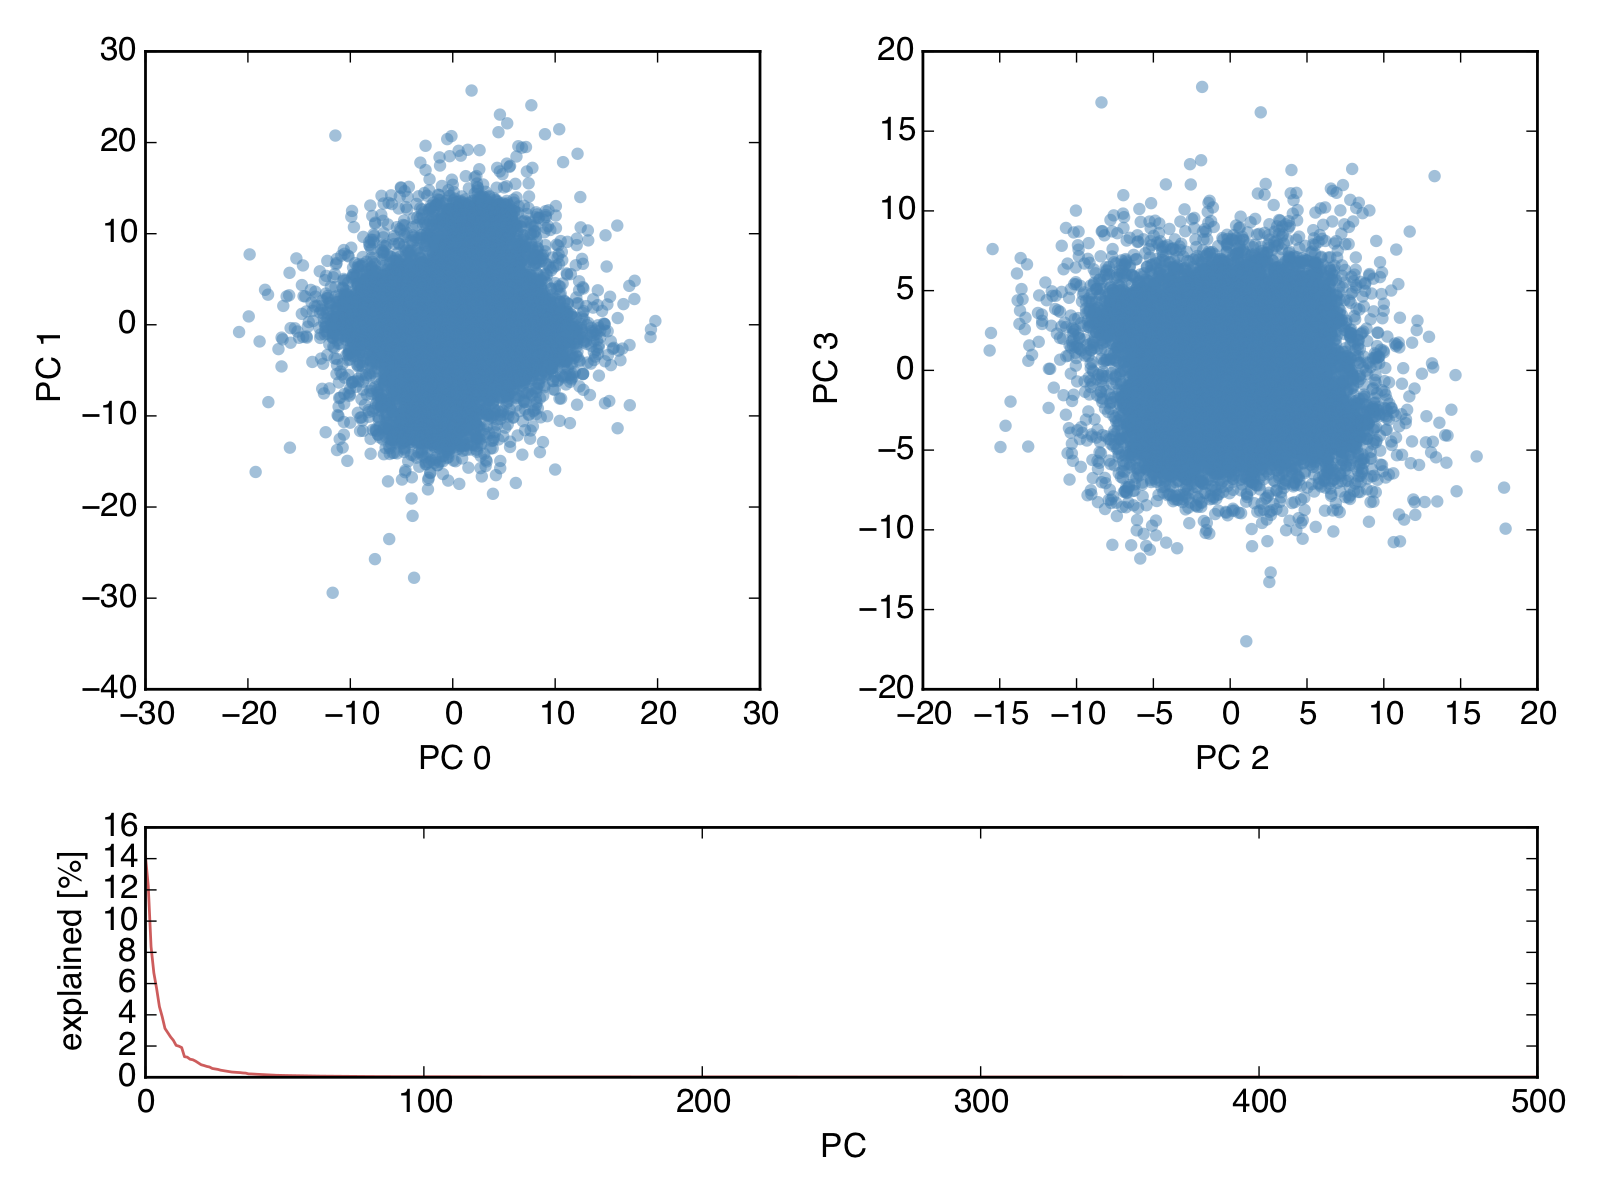
\includegraphics[width=0.9\textwidth]{results/doc2vec-pca}
	\caption{Document vectors calculated from just the title. Explained variance on the first 4 principal components is 41.4\%.}
\end{figure}

The explained variance is 41.4\% for the first 4 principal components, which may be higher than expected. This might be because word2vec part of the model, is quite good at guessing a missing word given just a short context. The big context which is what the document vector provides, may not be very important and only inform about the general rhetorical pattern. This could be (formal versus informal) or (angry versus happy). There thus exists a lower dimensional space there contains almost the same information as the 500 dimensional space.

\paragraph{Distance histogram} Again because the distance is used for clustering, the distance histogram is inspected. Furthermore the $0.1\%$ percentile is used for calculating the threshold $t$.

\begin{figure}[H]
        \centering
        \begin{subfigure}[b]{0.49\textwidth}
                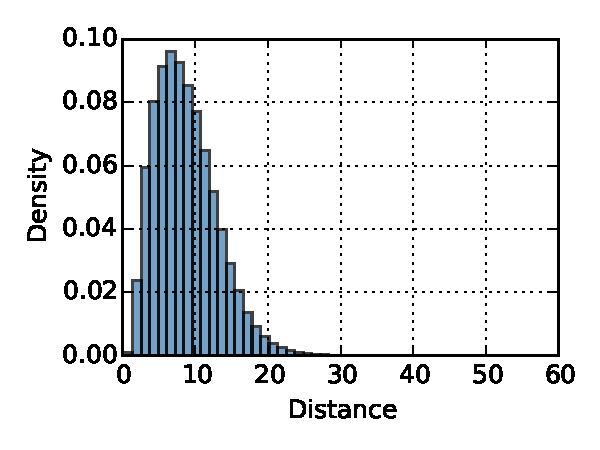
\includegraphics[width=\textwidth]{results/doc2vec-l2-histogram}
                \caption{Euclidean distance ($t \approx 1.35$)}
        \end{subfigure}
        \begin{subfigure}[b]{0.49\textwidth}
                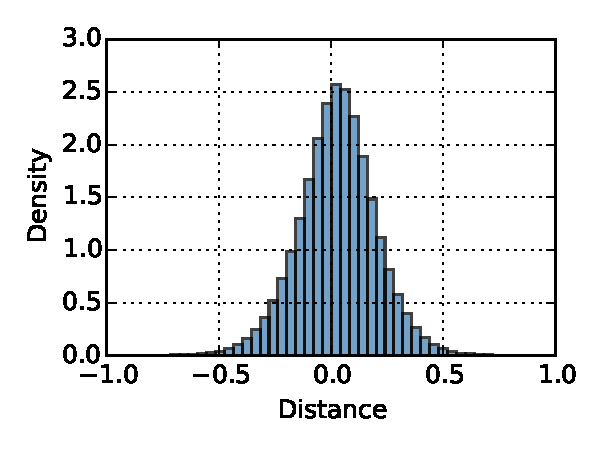
\includegraphics[width=\textwidth]{results/doc2vec-cos-histogram}
                \caption{Cosine similarity ($t \approx -0.66$)}
        \end{subfigure}
        \caption{Histograms of the distance between the document vectors.}
\end{figure}

The distance histograms are distribution wise a bit cleaner than in the skip-gram case. This is likely because the distribution of the document is more multivariate normal, at least when inspecting the PCA plots. This will of cause result a cleaner distribution in the distance as well.

The euclidean distance distribution looks like a gamma or $\chi^2$ distribution. This is likely because of the squaring in the distance calculation, which prevents the distance from becoming negative. In the skip-gram case this was less of an issue because the mean (relative to the standard deviance) was larger.

\paragraph{Inspecting clusters} From inspecting the clusters the result seem to be worse when comparing to the skip-gram case.

When inspecting the cluster distribution it turns out that with paragraph2vec, clustering with cosine similarity actually yields more reasonably sized clusters, compared to when the euclidean distance is used for clustering. This may be because of the $\chi^2$ like distribution of the euclidean distances, which makes it more difficult to separate articles about the same story from those about different stories. It's possible that a more fine-tuned threshold could yield better results, but in any case there still exists too small and way too big clusters.

\begin{table}[H]
\centering
\begin{tabular}{r|l l l l l l l }
size & 1 & 2 & 3 & 421 & 711 & 1855 & 3326 \\ \hline
amount & 93665 & 8 & 2 & 1 & 1 & 1 & 1
\end{tabular}
\caption{The cluster distribution using an euclidean distance shows unreasonably large and small clusters, and no reasonably or few reasonably sized clusters.}
\end{table}

Unfortunately the actual clusters that the clustering algorithm produces when using cosine similarity don't appear to capture any specific story. This is possibly because the document vectors only captures the overall mood of the article. For example the cluster in Table \ref{table:paragraph2vec:example} shows articles related to different bad events.

At last it was checked if the ``teenage stowaway'' cluster existed in this case. This should be a fairly easy set of article to cluster as it contains very specific word combinations. Unfortunately it didn't exists as a single cluster, which again indicates the document vectors only tells about the overall mood of the document, as a way of adjusting the word probabilities.

\begin{table}[H]
\centering
\begin{tabular}{r|p{10cm}}
id & title \\ \hline
  9489 & Ukraine crisis: Draft document reveals sanctions against Russian and Crimean officials \\
  6644 & Six Nations 2014: Stuart Lancaster hints at unchanged England \\
  7573 & US opens emergency oil stockpile in signal to Putin \\
  8998 & Saudi Arabia bans 50 ‘blasphemous’ and ‘inappropriate’ children’s names \\
  7862 & Rangers: Recovery on track after title win - Ally McCoist
\end{tabular}
\caption{Cluster example when using cosine similarity on the paragraph2vec results.}
\label{table:paragraph2vec:example}
\end{table}

